% This is LLNCS.DEM the demonstration file of
% the LaTeX macro package from Springer-Verlag
% for Lecture Notes in Computer Science,
% version 2.4 for LaTeX2e as of 16. April 2010
\documentclass{llncs}
\usepackage{array,multirow}
\usepackage{makeidx}  
\usepackage{rotating}
\usepackage{graphicx}
\graphicspath{{./Figures/OasisCor/},{./Figures/OasisRegression/},{./Figures/Ellipse/}}
\DeclareGraphicsExtensions{.pdf,.png}

\begin{document}

\title{Exploratory Population Analysis with Unbalanced Optimal Transport}
\titlerunning{Exploratory Population Analysis with Unbalanced Optimal Transport}  

\author{Samuel Gerber, Marc Niethammer, Martin Styner, Stephen Aylward}
\authorrunning{Gerber et al.} 
\institute{Kitware Inc, Carborro NC 27510, USA,\\
\email{samuel.gerber@kitware.com}
\and
University of North Carolina, Chapel Hill NC 27504, USA}


\maketitle              

% What problems are we addressing?
%  - [MRI] disentangle mass from shape changes
%  - [MRI] No segmentations needed
%  - [VESSELS] unstructured point clouds
%  - [VESSELS] background blood perfusion

% What's new?
%  - Hypothesis generation
%  - Different measure to capture changes
%  - No deformable registration
%  - No parameter tuning
%  - [MRI] Unbalanced mass transport
%  - [VESSELS] Decomposition of transport plan with respect to underlying measure


\begin{abstract}
The plethora of data from neuroimaging studies provide a rich opportunity to
discover effects and generate hypotheses through exploratory data analysis. The
pathologies in brain disease often manifest in changes in shape along with
deterioration and alteration of brain matter, i.e. changes in mass. We propose
to use unbalanced optimal transport to disentangle shape from mass changes and
localize those changes. The exploratory analysis approach generates images of
transport cost and mass changes for each subject in the population.  Using
voxelwise correlations with disease indicators on these images highlight
regions of interest in mass or shape changes related to the disease indicator.
We demonstrate the method on the white and gray matter segmentations from the
OASIS brain MRI data set, which includes subject ranging from healthy to mild
and moderate dementia. The results corroborate known pathology changes related
to dementia and suggest avenues for further clinical research. Additionally
regression and permutation testing on the transport cost and mass change images
improve on existing methods to predict disease measures and indicates that the
proposed method captures a larger portion of the pathology induced changes.  
\end{abstract}

\section{Introduction}
\begin{figure}
\centering
\begin{tabular}{c|c}
\begin{tabular}{cc}

\includegraphics[width=0.1\linewidth]{ellipse0001} &

\includegraphics[width=0.1\linewidth]{ellipse0002} \\

\includegraphics[width=0.1\linewidth]{ellipse0003} &

\includegraphics[width=0.1\linewidth]{ellipse0004} \\

\includegraphics[width=0.1\linewidth]{ellipse0005} &

\includegraphics[width=0.1\linewidth]{ellipse0006} \\
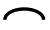
\includegraphics[width=0.1\linewidth]{ellipse0007} &
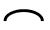
\includegraphics[width=0.1\linewidth]{ellipse0008} \\
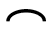
\includegraphics[width=0.1\linewidth]{ellipse0009} & 
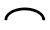
\includegraphics[width=0.1\linewidth]{ellipse0010} \\ 
\end{tabular}
        &
\begin{tabular}{l|c|c|c}
Intensity&
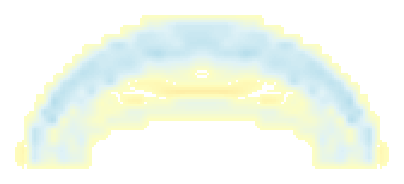
\includegraphics[width=0.2\linewidth]{cor-mass-intensity} &
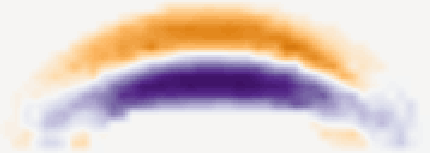
\includegraphics[width=0.2\linewidth]{cor-rx-ry-intensity} &
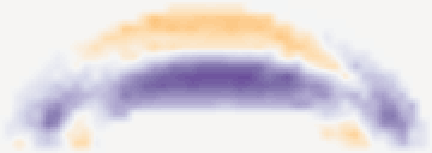
\includegraphics[width=0.2\linewidth]{cor-rx-ry-mass-intensity} \\ \hline
Mass&
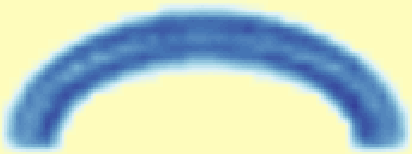
\includegraphics[width=0.2\linewidth]{cor-mass-mass} &
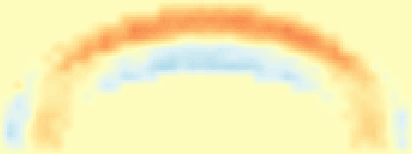
\includegraphics[width=0.2\linewidth]{cor-rx-ry-mass} &
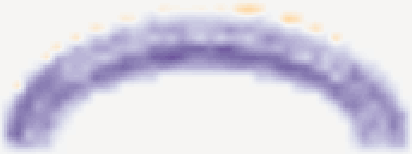
\includegraphics[width=0.2\linewidth]{cor-rx-ry-mass-mass} \\
Cost&
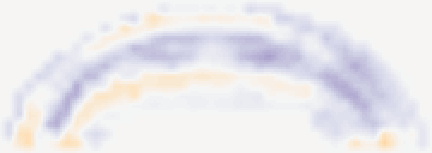
\includegraphics[width=0.2\linewidth]{cor-mass-cost} &
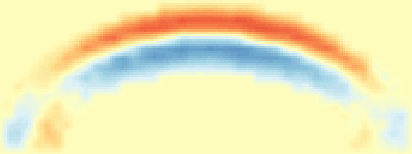
\includegraphics[width=0.2\linewidth]{cor-rx-ry-cost} &
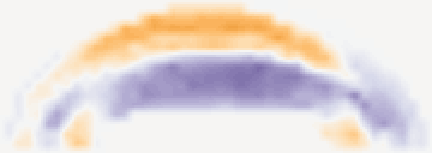
\includegraphics[width=0.2\linewidth]{cor-rx-ry-mass-cost} \\ \hline \hline
        & Size & Ellipticity & Ellipticity + Size
\end{tabular} \\
        (a) & (b)
\end{tabular}
\caption{\label{fig:cor-ellipse}
Illustration of unbalanced optimal transport on a (a) toy data set of a 100
ellipses with different minor and major radii and width.  (b) Correlation
of total size (number of black pixels), ellipticity (ratio of the minor and major radii)
and sum of size and ellipticity (top) to raw pixel intensity values, (middle)
optimal transport mass imbalances and (bottom) optimal transport costs. The
optimal transport approach correctly identifies changes in size in the mass
imbalance with stronger correlations than the intensity based approach.
Ellipticity is strongly captured in both the optimal transport cost and
the intensity. Some of the ellipticity is also captured in the optimal
transport mass since larger radii also correlate with an increase in
size. Correlation to an additive shape and mass effect are correctly
identified as in both the optimal transport cost and mass imbalance,
while the intensity values alone lead to weaker correlation without any
indicator of the driving changes.   }
\end{figure}

\section{Background}

\subsection{Population Analysis}

\subsection{Optimal Transport}

\section{Optimal Transport for Population Analysis}

\section{Application to OASIS Brain MRI}

\begingroup
\renewcommand{\arraystretch}{0}
\setlength{\tabcolsep}{0pt}
\begin{figure}[!b]
\centering
\begin{tabular}{l|cc|cc|cc} 
\parbox[t]{4mm}{\multirow{3}{*}{\rotatebox[origin=c]{90}{Mass Imbalance}}}&
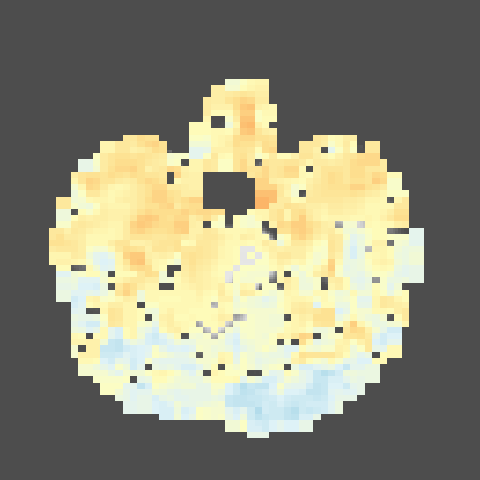
\includegraphics[width=0.16\linewidth]{cor-axial-age-mW} &
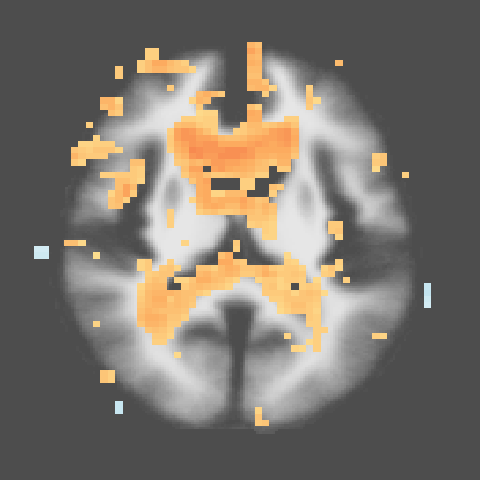
\includegraphics[width=0.16\linewidth]{cor-axial-age-t-mW} &
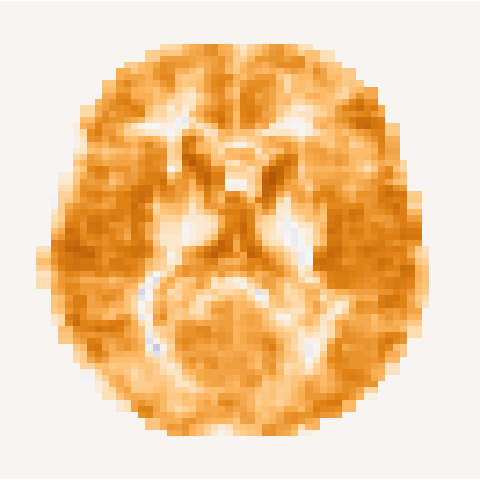
\includegraphics[width=0.16\linewidth]{cor-axial-cdr-mW} &
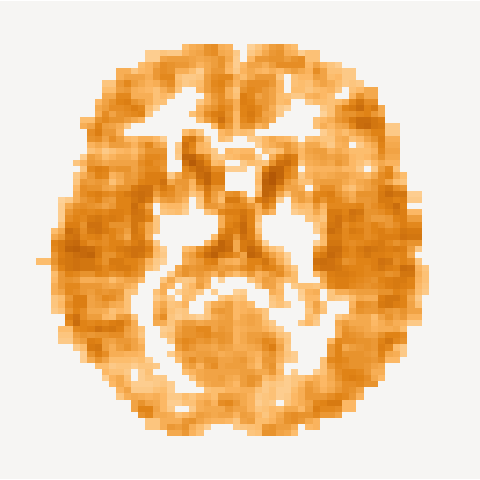
\includegraphics[width=0.16\linewidth]{cor-axial-cdr-t-mW} &
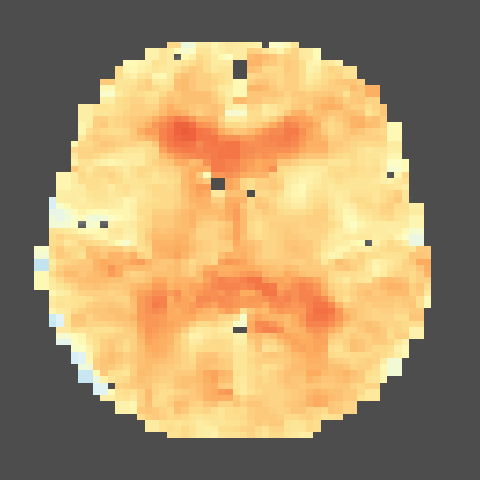
\includegraphics[width=0.16\linewidth]{cor-axial-mmse-mW} &

\includegraphics[width=0.16\linewidth]{cor-axial-mmse-t-mW} \\ 
%
        &
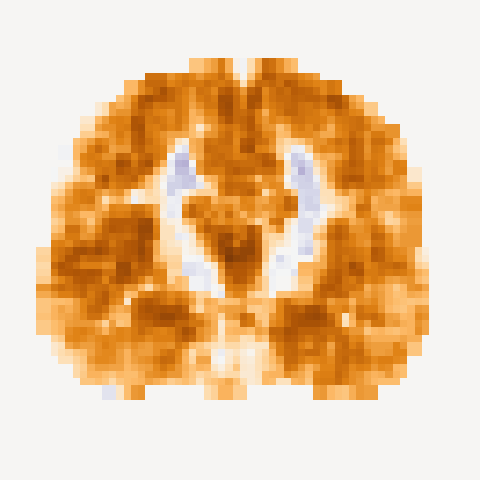
\includegraphics[width=0.16\linewidth]{cor-coronal-age-mW} &
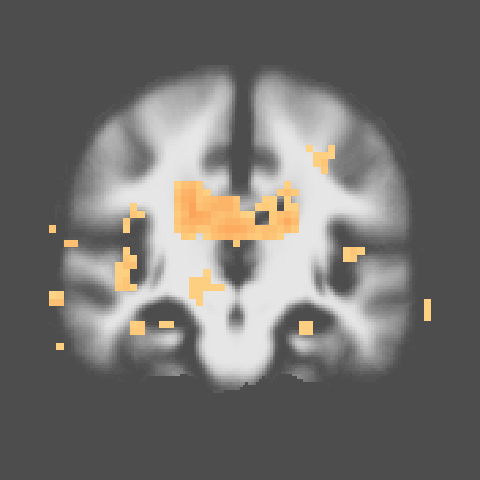
\includegraphics[width=0.16\linewidth]{cor-coronal-age-t-mW} &
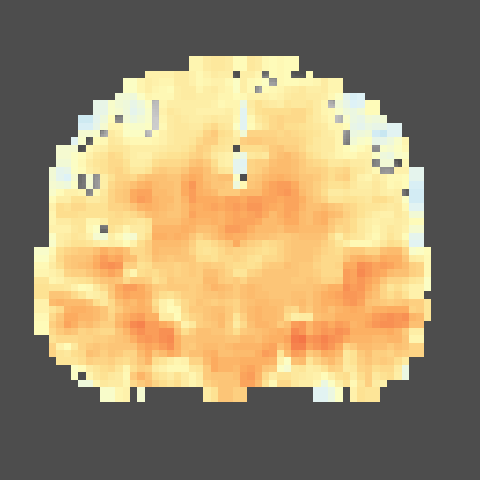
\includegraphics[width=0.16\linewidth]{cor-coronal-cdr-mW} &
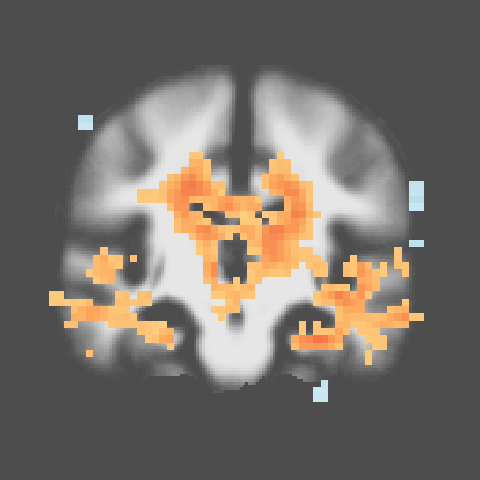
\includegraphics[width=0.16\linewidth]{cor-coronal-cdr-t-mW} &
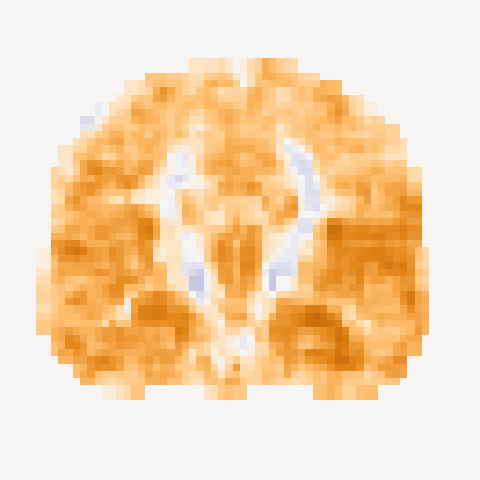
\includegraphics[width=0.16\linewidth]{cor-coronal-mmse-mW} &
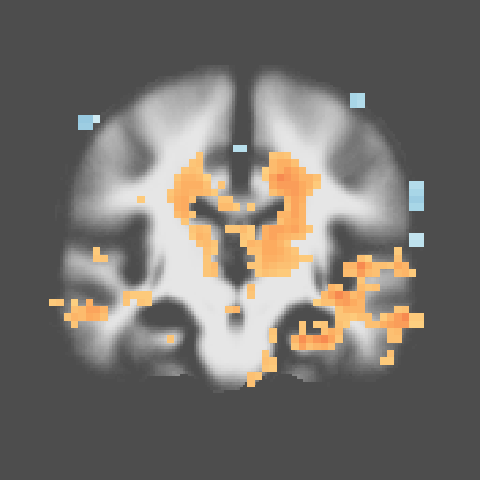
\includegraphics[width=0.16\linewidth]{cor-coronal-mmse-t-mW} \\ 
%
        &
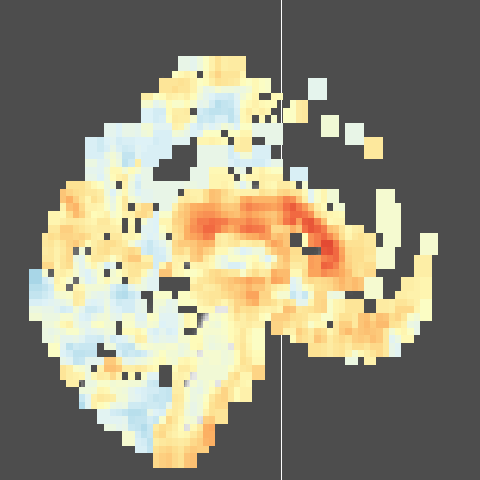
\includegraphics[width=0.16\linewidth]{cor-sagital-age-mW} &
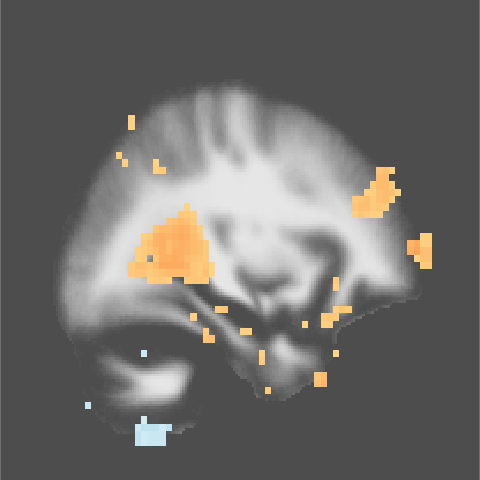
\includegraphics[width=0.16\linewidth]{cor-sagital-age-t-mW} &
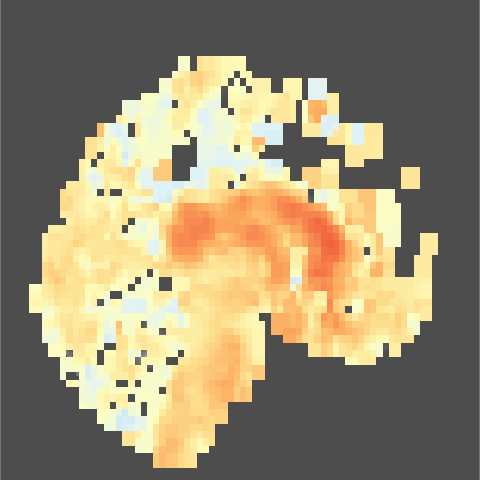
\includegraphics[width=0.16\linewidth]{cor-sagital-cdr-mW} &
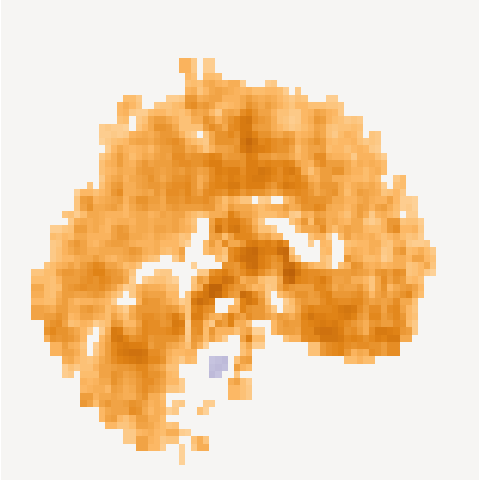
\includegraphics[width=0.16\linewidth]{cor-sagital-cdr-t-mW} &
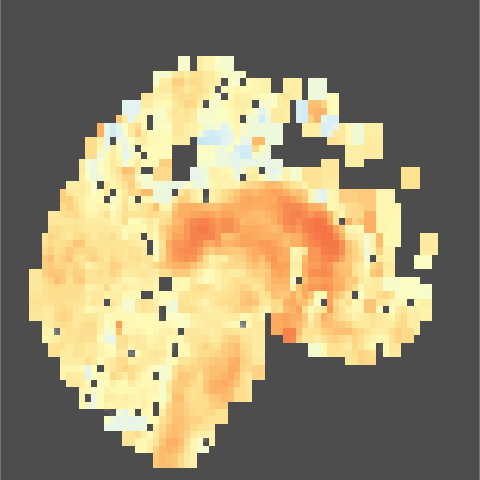
\includegraphics[width=0.16\linewidth]{cor-sagital-mmse-mW} &
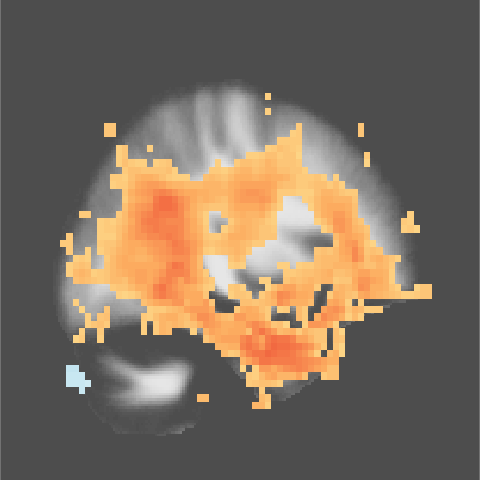
\includegraphics[width=0.16\linewidth]{cor-sagital-mmse-t-mW} \\ \hline \hline
%
\parbox[t]{2mm}{\multirow{3}{*}{\rotatebox[origin=c]{90}{Transport Cost}}}&
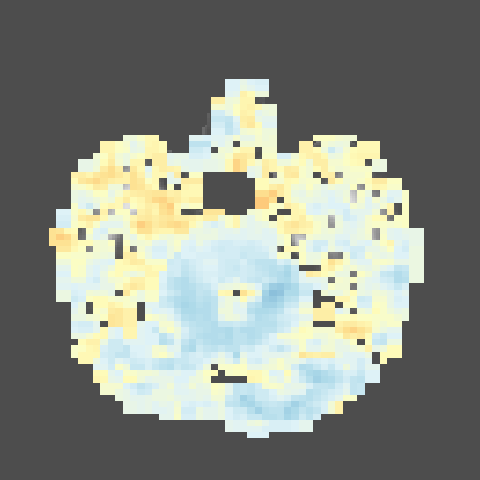
\includegraphics[width=0.16\linewidth]{cor-axial-age-tW} &
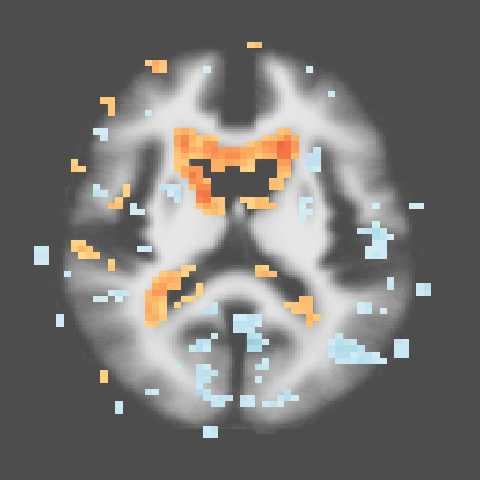
\includegraphics[width=0.16\linewidth]{cor-axial-age-t-tW} &
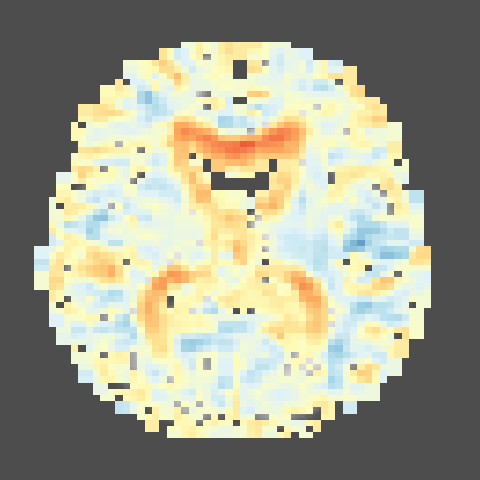
\includegraphics[width=0.16\linewidth]{cor-axial-cdr-tW} &
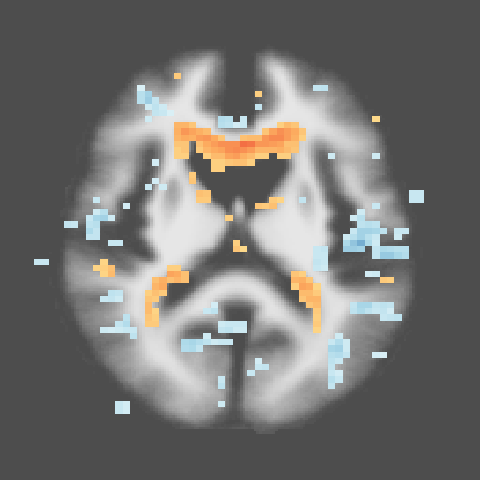
\includegraphics[width=0.16\linewidth]{cor-axial-cdr-t-tW} &
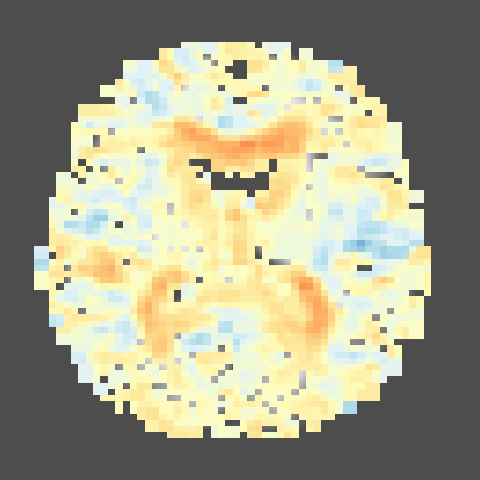
\includegraphics[width=0.16\linewidth]{cor-axial-mmse-tW} &
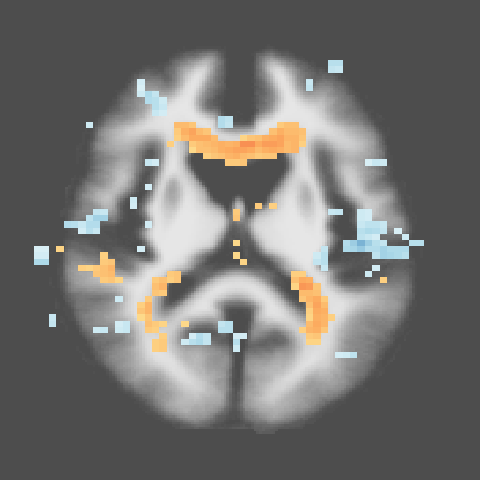
\includegraphics[width=0.16\linewidth]{cor-axial-mmse-t-tW} \\ 
%
        &
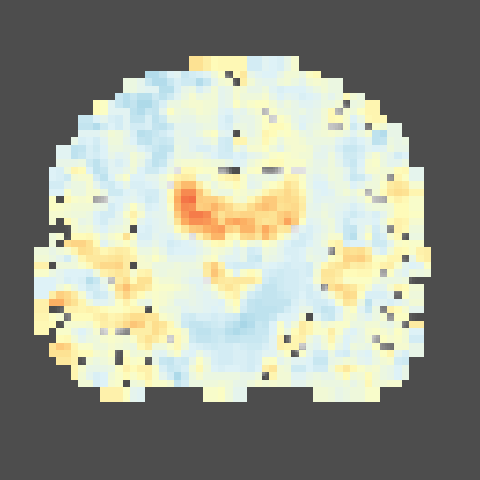
\includegraphics[width=0.16\linewidth]{cor-coronal-age-tW} &
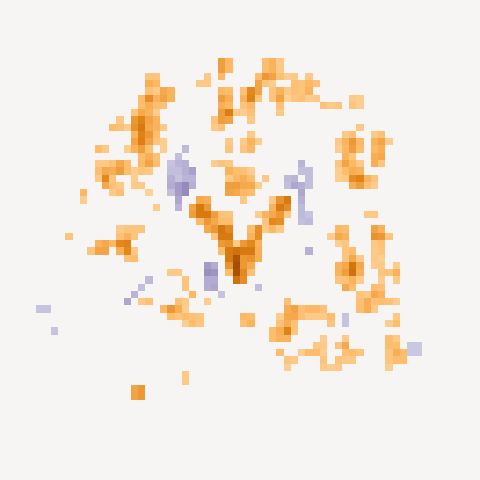
\includegraphics[width=0.16\linewidth]{cor-coronal-age-t-tW} &
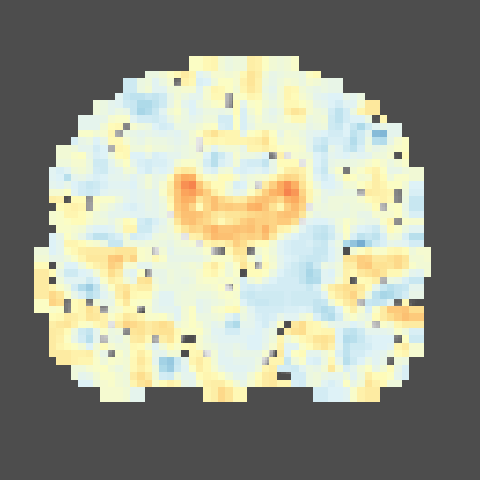
\includegraphics[width=0.16\linewidth]{cor-coronal-cdr-tW} &
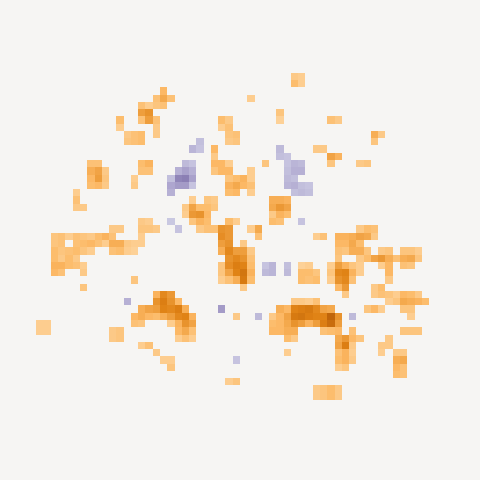
\includegraphics[width=0.16\linewidth]{cor-coronal-cdr-t-tW} &
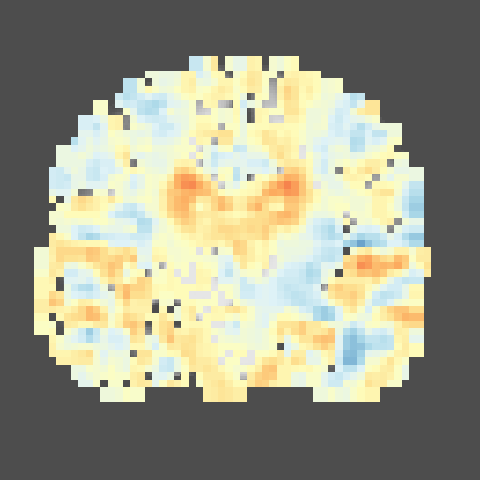
\includegraphics[width=0.16\linewidth]{cor-coronal-mmse-tW} &
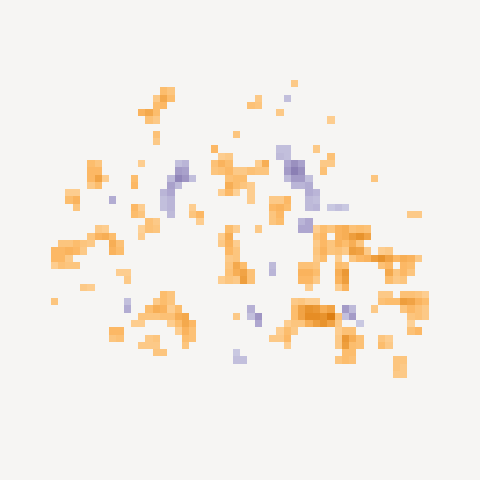
\includegraphics[width=0.16\linewidth]{cor-coronal-mmse-t-tW} \\ 
%
        &
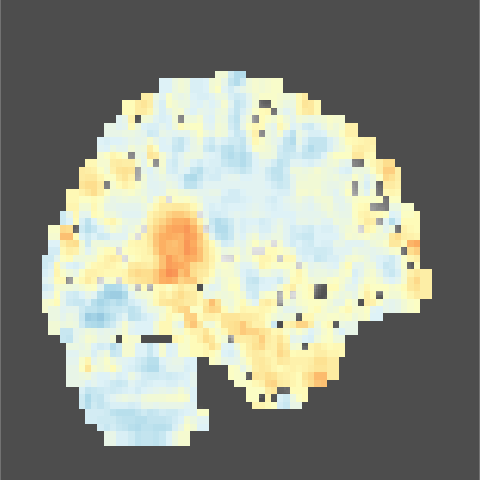
\includegraphics[width=0.16\linewidth]{cor-sagital-age-tW} &
\includegraphics[width=0.16\linewidth]{cor-sagital-age-t-tW} &
\includegraphics[width=0.16\linewidth]{cor-sagital-cdr-tW} &
\includegraphics[width=0.16\linewidth]{cor-sagital-cdr-t-tW} &
\includegraphics[width=0.16\linewidth]{cor-sagital-mmse-tW} &
\includegraphics[width=0.16\linewidth]{cor-sagital-mmse-t-tW} \\ \hline \hline
%
& \parbox[b][4mm]{6mm}{Age} 
& \parbox[b][4mm]{6mm}{Age\textsuperscript{*}} 
& \parbox[b][4mm]{6mm}{CDR} 
& \parbox[b][4mm]{6mm}{CDR\textsuperscript{*}}
& \parbox[b][4mm]{6mm}{MMSE}
& \parbox[b][4mm]{6mm}{MMSE\textsuperscript{*}}
\end{tabular}
\caption{\label{fig:cor-oasis-white}
Correlation of age, MMSE and CDR with optimal transport mass imbalances and
optimal transport costs of white matter. The columns with a \textsuperscript{*}
only show the voxels were the correlation has a permutation tested p-value less
than 0.05  }
\end{figure}
\endgroup

\begingroup
\renewcommand{\arraystretch}{0}
\setlength{\tabcolsep}{0pt}
\begin{figure}[!b]
\centering
\begin{tabular}{l|cc|cc|cc}
\parbox[t]{4mm}{\multirow{3}{*}{\rotatebox[origin=c]{90}{Mass Imbalance}}}&
\includegraphics[width=0.16\linewidth]{cor-axial-age-mG} &
\includegraphics[width=0.16\linewidth]{cor-axial-age-t-mG} &
\includegraphics[width=0.16\linewidth]{cor-axial-cdr-mG} &
\includegraphics[width=0.16\linewidth]{cor-axial-cdr-t-mG} &
\includegraphics[width=0.16\linewidth]{cor-axial-mmse-mG} &
\includegraphics[width=0.16\linewidth]{cor-axial-mmse-t-mG} \\ 
%
        &
\includegraphics[width=0.16\linewidth]{cor-coronal-age-mG} &
\includegraphics[width=0.16\linewidth]{cor-coronal-age-t-mG} &
\includegraphics[width=0.16\linewidth]{cor-coronal-cdr-mG} &
\includegraphics[width=0.16\linewidth]{cor-coronal-cdr-t-mG} &
\includegraphics[width=0.16\linewidth]{cor-coronal-mmse-mG} &
\includegraphics[width=0.16\linewidth]{cor-coronal-mmse-t-mG} \\ 
%
        &
\includegraphics[width=0.16\linewidth]{cor-sagital-age-mG} &
\includegraphics[width=0.16\linewidth]{cor-sagital-age-t-mG} &
\includegraphics[width=0.16\linewidth]{cor-sagital-cdr-mG} &
\includegraphics[width=0.16\linewidth]{cor-sagital-cdr-t-mG} &
\includegraphics[width=0.16\linewidth]{cor-sagital-mmse-mG} &
\includegraphics[width=0.16\linewidth]{cor-sagital-mmse-t-mG} \\ \hline \hline
%
\parbox[t]{2mm}{\multirow{3}{*}{\rotatebox[origin=c]{90}{Transport Cost}}}&
\includegraphics[width=0.16\linewidth]{cor-axial-age-tG} &
\includegraphics[width=0.16\linewidth]{cor-axial-age-t-tG} &
\includegraphics[width=0.16\linewidth]{cor-axial-cdr-tG} &
\includegraphics[width=0.16\linewidth]{cor-axial-cdr-t-tG} &
\includegraphics[width=0.16\linewidth]{cor-axial-mmse-tG} &
\includegraphics[width=0.16\linewidth]{cor-axial-mmse-t-tG} \\ 
%
        &
\includegraphics[width=0.16\linewidth]{cor-coronal-age-tG} &
\includegraphics[width=0.16\linewidth]{cor-coronal-age-t-tG} &
\includegraphics[width=0.16\linewidth]{cor-coronal-cdr-tG} &
\includegraphics[width=0.16\linewidth]{cor-coronal-cdr-t-tG} &
\includegraphics[width=0.16\linewidth]{cor-coronal-mmse-tG} &
\includegraphics[width=0.16\linewidth]{cor-coronal-mmse-t-tG} \\ 
%
        &
\includegraphics[width=0.16\linewidth]{cor-sagital-age-tG} &
\includegraphics[width=0.16\linewidth]{cor-sagital-age-t-tG} &
\includegraphics[width=0.16\linewidth]{cor-sagital-cdr-tG} &
\includegraphics[width=0.16\linewidth]{cor-sagital-cdr-t-tG} &
\includegraphics[width=0.16\linewidth]{cor-sagital-mmse-tG} &
\includegraphics[width=0.16\linewidth]{cor-sagital-mmse-t-tG} \\ \hline \hline
%%
& \parbox[b][4mm]{6mm}{Age} 
& \parbox[b][4mm]{6mm}{Age\textsuperscript{*}} 
& \parbox[b][4mm]{6mm}{CDR} 
& \parbox[b][4mm]{6mm}{CDR\textsuperscript{*}}
& \parbox[b][4mm]{6mm}{MMSE}
& \parbox[b][4mm]{6mm}{MMSE\textsuperscript{*}}
\end{tabular}
\caption{\label{fig:cor-oasis-white}
Correlation of age, MMSE and CDR with optimal transport mass imbalances and
optimal transport costs of white matter. The columns with a \textsuperscript{*}
only show the voxels were the correlation has a permutation tested p-value less
than 0.05  }
\end{figure}
\endgroup




\section{Conclusion}

- Localized mass preserving
- Clustering

\end{document}
